%This document demonstrates proper use of REV\TeX~4 (and
%\LaTeXe) in mansucripts prepared for submission to APS
%journals. Further information can be found in the REV\TeX~4
%documentation included in the distribution or available at
%\url{http://publish.aps.org/revtex4/}. 
% TeX'ing this file requires that you have AMS-LaTeX 2.0 installed
% as well as the rest of the prerequisites for REVTeX 4.0 .
% If you compile your tex files on the Physics
% server, everything is already set up for you.
%

% Choose the format that suits your purposes.  The top line gives the
% two column (twocolumn) format that one sees in printed journals.  The
% second line refers to a one column double spaced format (preprint) that
% is useful during editing.  Use the "%" symbol to edit out the line
% you do not want to use.

\documentclass[draft, twocolumn,showpacs,preprintnumbers,amsmath,amssymb]{revtex4}
%\documentclass[preprint,showpacs,preprintnumbers,amsmath,amssymb]{revtex4}
% Additional packages needed for graphics, alignment and math fonts.

\usepackage{graphicx}% Include figure files in eps format.
\usepackage{dcolumn}% Align table columns on decimal point.
\usepackage{bm}% bold math.

% The \begin{document} command set the start of the RevTeX commands.

\begin{document}

\title{Identification and Quantification of Diffusion MRI Biomarkers to Study Spinal Cord Injury}

\author{Marcus Lee}
\email{marcus99@student.ubc.ca}
\affiliation{Department of Physics and Astronomy, University of British Columbia \\
             6224 Agricultural Road, Vancouver, British Columbia, Canada, V6T 1Z1}

\date{\today}

\begin{abstract}
Provide a brief summary of the proposal here. This  should be a concise  
statement of what will be accomplished, the methods that will be used, and the potential significance. Many of you have already sent me a description of the project that can be put here with some  touching up. I will only  accept LATEX complied files in pdf format. They must be emailed to me a few days  before the oral presentations.  Make sure your supervisor has a chance to read it over before you hand it in. 

\end{abstract}

\maketitle

% The first section of the paper.

\section{Motivation}
% The value in studying spinal cord injuries
    % The value in terms of identifying Bio markers
% Some modern biomarkers that could be identified
% The value in terms of reducing the space of histologies
% Finding the biomarkers will reduce the space of relevant histologies
% The value in terms of imporving MRI analysis
% A more direct statement on what we hope to find and the impact of that

\sci is a major focus of neuropathology research where despite recent progress in neuroscience most patients experiencing \sci are unlikely to make a full recovery and instead experience neurological loss as well as other complications. Given the infrequency of recovery, accurate and reproducible objective indicators of a patient's health, known as biomarkers are necessary to conduct ethical and practical clinical trials and therefore any correlations between biomarkers and the degree of injury is of great research interest. Additionally, some biomarkers may track tissue changes following \sci which will provide value in predicting the severity and the recovery. \cite{hulme2017developing} Identifying practical sensitive and non-invasive biomarkers will reduce the high cost associated with assessing the severity of \sci by limiting the number of imaging tests needed to determine appropriate treatment and ensuring any intervention is better personalized to the patient. \cite{badhiwala2018review}

\if{false}
- There aren't good treatments for sci in general %

- As a general feature of biomarkers finding them allows for more quantitative treatment of pathologies and shorter more ethical trials%

- Biomarkers are also a good measure for predicting recovery and setting expectations for outcomes%

- The discovery and validation of biomarkers has benefits see notes%

- Measurement of injured spinal cord histologies will allow us to properly connect the biomarkers to the structural damage to the actual clincal outcomes which in our case is the eventual death of the patient due to their injuries.%

- In particular see notes for the possible biomarkers that could be indicative of structural problems in the spinal cord that could be found as a result of our research%

- Biomarkers are objectively quantifiable indicators of the medical state of a patient that can be measured from the outside.
\fi%

A potential source of biomarkers that indicate structural damage to the spinal cord would be a disruption in the \bscb that causes cellular materials from the injury site can spill into the \csf or blood, alternatively one can look for signs of pathological functions such as inflammation. The identity of these components could signify damage to neuronal cells. One example of a theoretical biomarker is \gfap which is a protein only found within astroglial cells that play a role in the development of the cytoskeleton's glial cells and its production is stimulated in response to \sci where within the first 24-hours post-injury there is no significant correlation between injury grade and \gfap concentrations \cite{pouw2014structural} however within 72-hours \gfap concentrations are correlated with severity \cite{kwon2010cerebrospinal, ahadi2015diagnostic} and analysis of \gfap in \csf predicted \sci severity and recovery outcomes with 83\% accuracy. \cite{kwon2017cerebrospinal}

\if{false}
\mbp is a major component of myelin which is a fatty material that electrically insulates axons which themselves make up a majority of white matter and the spinal cord. Demyelination is a symptom Multiple Sclerosis and also occurs from the severing of axons form the body of the neurons. \mbp can be found concentrated near new oligodendrocytes and is a potential biomarker for remyelination. \cite{hesp2015chronic, zhang2011neurological}
\fi

% Maybe write something about macrophage inflammatory protiens (MIPs)

% Still need to make a point about finding the correlations between them and verifying a causation

\if{false}
Many studies into potential biomarkers are limited by a lack of human studies \cite{badhiwala2018review} and animals such as rodents have structurally simpler nervous systems with different recovery trends compared to humans. \cite{courtine2007can}
\fi

\mri is an essential tool for diagnosing and determining the rehabilitation \sci in patients. \mri methods that allow the mapping of the spinal cord histologies in patients with \sci will aid in determining causation from potential biomarkers as well as the investigation of biomarkers derived from the \mri parameters. \cite{freund2016embodied} The use of \mri for prognosis is preferable because it avoids the negative effects of imaging techniques that make use of ionizing radiation and it is non-invasive unlike methods involving the collection of \csf which adds the risk of patient pain and spinal cord compression. \cite{hrishi2019cerebrospinal} Quantitative \mri techniques such as \dmri enable probing of the spinal cord microstructure for features orders of magnitude smaller than the voxel size \mri scan by measuring the directional diffusion of water inside the tissue, this allows for more precise detection of metrics such as demyelination and tissue integrity. \cite{cohen2018microstructural, cadotte2018has, freund2013mri, seif2018quantitative}

Extracting the spinal cord histology from the \dmri data requires assuming a mathematical model of the underlying tissue and fitting the data to it. A common technique known as \dti models the diffusivity with a single tensor in each voxel and the histology is interpreted from \dti metrics such as using fractional anisotropy, a quantity derived from the tensor eigenvalues, to quantify axon pathology. \dti techniques are limited by unrealistic assumptions such as modelling the region as a single compartment with no fibre crossing or dispersion \cite{vedantam2014diffusion} more advanced biophysical models that account for the inhomogeneity of the tissue such as NODDI and ActiveAx are computationally complex, degenerate in their parameters, and research studies are needed to determine fitting constraints as well as explicitly describe appropriate fixed parameter values. One obstacle to this is difficulty separating degrees of freedom in the model from biological variability in patients yielding poorly understood outcomes. \cite{novikov2018modeling}

This project will combine 32 metrics in 50 spinal cord segments allowing us to map diffusion parameters across the length of many spinal cords enabling us to measure the correlations between them which have the potential to greatly reduce the space possible parameters in biophysical models and their associated histologies. Our results will provide useful insight into theorized biomarkers and inform future studies utilizing in vivo measurements. 

% DMRI to probe the microstructure + defining DMRI
% DMRI to improve over conventional MRI
% Recent advancements in image processing to make DMRI feasible
% Reduction of the parameter space for biophysical models that correspond to real SCI
% Direct statement on what we want to find (A this project statement)





In this section introduce the subject of the proposal and  provide all the necessary background information that will be needed for a {\bf non-expert} to understand.  This  should involve reading at least 5-10 journal articles some of which your supervisor will likely provide and others you will need to look up. These should all be listed in the bibliography. 
Items in the bibliography can be referenced  as follows. The text inside the curly brackets are
used to label the references. Numbers appear automatically in the compiled
text.

Most importantly you must provide  the scientific motivation for why this project should be carried out and what scientific impact it could have if  it were completely successful. Any research project requires a substantial  investment of resources (money for equipment, use of common facilities, computer time for calculations/data analysis, the countless hours spent by you and your supervisor etc.) You must convince  the reader/reviewer that the project and the potential outcome is worth this investment. Imagine that only a fraction of the  proposals submitted will be approved. If yours is not approved then you must rework the proposal or find another project for which the scientific justification is stronger.  This is typical of the competitive  environment one is often faced with in research. There is always  a demand for  resources and/or access to facilities which exceeds the availability.  Only the best projects get funded or receive time on a facility (e.g. telescope or accelerator). It is  your responsibility to make the case that your proposal  should be  approved. In this case I am the reviewer who decides if you get approval.

\section{Theory}
% NMR / MRI Theory
% DMRI Theory and measurement
% Using Biophysical Models to make sense of MRI data through essentially solving for fit parameters

% ^^ This will be more than enough content

%\subsection{Nuclear Magnetic Resonance}

\subsection{Magnetic Resonance Imaging}
\mri is the use of nuclear magnetic resonance to probe the structure of a sample. Protons neutrons are particles with a non-zero spin angular momentum therefore ground state nuclei containing an odd number of protons have a net magnetic moment and in the presence of a magnetic field there is a lifting of the degeneracy of the spin-up and spin-down magnetic substates causing it to be energetically preferable for the spins of the particles to be oppositely aligned, this is known as the Zeeman effect, the energy splitting is given by equation \ref{eq:zeeman}.
\begin{equation}
    \Delta E = \gamma \mu B_0
    \label{eq:zeeman}
\end{equation}

Where $B_0$ is the strength of the applied magnetic field, $\mu$ is the nuclear magneton, and $\gamma$ is the gyrometric factor which depends on the angular momentum of the particle. \cite{griffiths2005introduction} In practice, nuclei feel the external field and internal fields from chemical bonding causing a shift in $\Delta E$ and these shifts are catalogued into functional groups. If we consider a proton rich sample individual protons can emit and absorb photons that match the energy splitting to transition between states, the energy splitting can be determined from measuring the absorption spectrum of the sample where the most energy will be absorbed at the frequency that matches $\Delta E$, this effect is known as nuclear magnetic resonance. \cite{bushberg2011essential} The total energy absorbed is proportional to the number of protons that have been excited therefore when $\Delta E$ is known, a non uniform $\vec{B}$ field can be applied such that the sample will only resonate with the sample in a single plane, choosing a plane is known slice selection, measuring the absorbed energy we learn the proton density in that slice.

Another observable signal is the photons released by the protons as the sample lose magnetization and relaxes back to thermal equilibrium. The time change in magnetization, $\vm$, is given by the equation \ref{eq:bloch} the Bloch equation where we assume $\vec{B_0}$ is pointing along the z-axis:

\begin{equation}
    \frac{d \vm}{dt} = \gamma \vm \times \vec{B_0} - \frac{M_x \hat{x} + M_y \hat{y}}{T_2^*} - \frac{M_z - M_0}{T_1}\hat{z}
    \label{eq:bloch}
\end{equation}

Where $M_0$ is the z-component at thermal equilibrium, $T_1$ is the spin-lattice relaxation constant, and $T_2^*$ is the spin-spin relaxation constant and depend on the structure of the tissue. \cite{bushberg2011essential} Sequences of radio frequency pulses can be used to flip the magnetic moments of the protons and then a gradient can then be applied within the slice to cause the magnetic moments to precess at specific frequencies and phases, this information is encoded in the radio signals produced during relaxation and the measured \mr signals form a k-space matrix of which the Fourier transform yields the real space image of the sample.


% The photon energy has to match the energy splitting

% This preferential absorption spectrum is known as nuclear magnetic resonance

% From NMR, and prior knowledge of the absorption frequency we choose a non uniform B field such that resonance condition is only met in a small region usually a plane. The energy absorbed can be measured with a pickup coil

\subsection{Diffusion MRI}
% Maybe say something about the fundamental limits of conventional MRI
% I have to define all or most of the parameters that the following models depend on

Equation \ref{eq:bloch} assumed stationary protons, if we consider the fact that the protons have the ability to diffuse then we modify equation \ref{eq:bloch} to get equation \ref{eq:torrey} the Bloch-Torrey equation:

\begin{equation}
    \frac{d \vm}{dt} = \frac{d \vm_{\text{Bloch}}}{dt} + \nabla \cdot D \nabla \vm
    \label{eq:torrey}
\end{equation}

Where ${d \vm_{\text{Bloch}}}/{dt}$ is the RHS of equation \ref{eq:bloch} and $D$ is the diffusion tensor. \cite{rohmer2006bloch}

% We will define and assume gaussian diffusion for this section.

The solution to this equation can be simplified as:

\begin{equation}
    \vm = \vm_{\text{Bloch}} e^{-\gamma^2 \delta^2_d \Delta \vec{G}^T D \vec{G}}
    \label{eq:bt_sol}
\end{equation}

Where $\Delta$ is the time between the beginning of each gradient pulse, $\delta_d$ is the length of the pulse, and $\vec{G}$ is the gradient applied to the slice. The factors in the exponent of equation \ref{eq:bt_sol} can be combined into a single factor, $b$, and used as a measure of the sequence's sensitivity to diffusion in the sample by defining:

\begin{equation}
    b = \gamma^2 \int_0^{TE} \int_0^t G(t') dt' dt
\end{equation}

Where $TE$ is the echo time which is the time between the exciting pulse and the measured signal. When time between pulses in an MRI sequence is long enough for diffusion to have a significant effect on the magnetization of the sample the dephasing pulse will no longer be rephased because diffusion will have changed the positions of the protons and therefore the phase difference in the slice will be proportional to the distance the protons have travelled. The effect of diffusion on the phase of the magnetic moments are illustrated in figure \ref{fig:phase} and the quantities $TE$, $\vec{G}$, $\delta_d$, and $\Delta$ are visualized in for a \dmri sequence in figure \ref{fig:sequence}.

\begin{figure}
    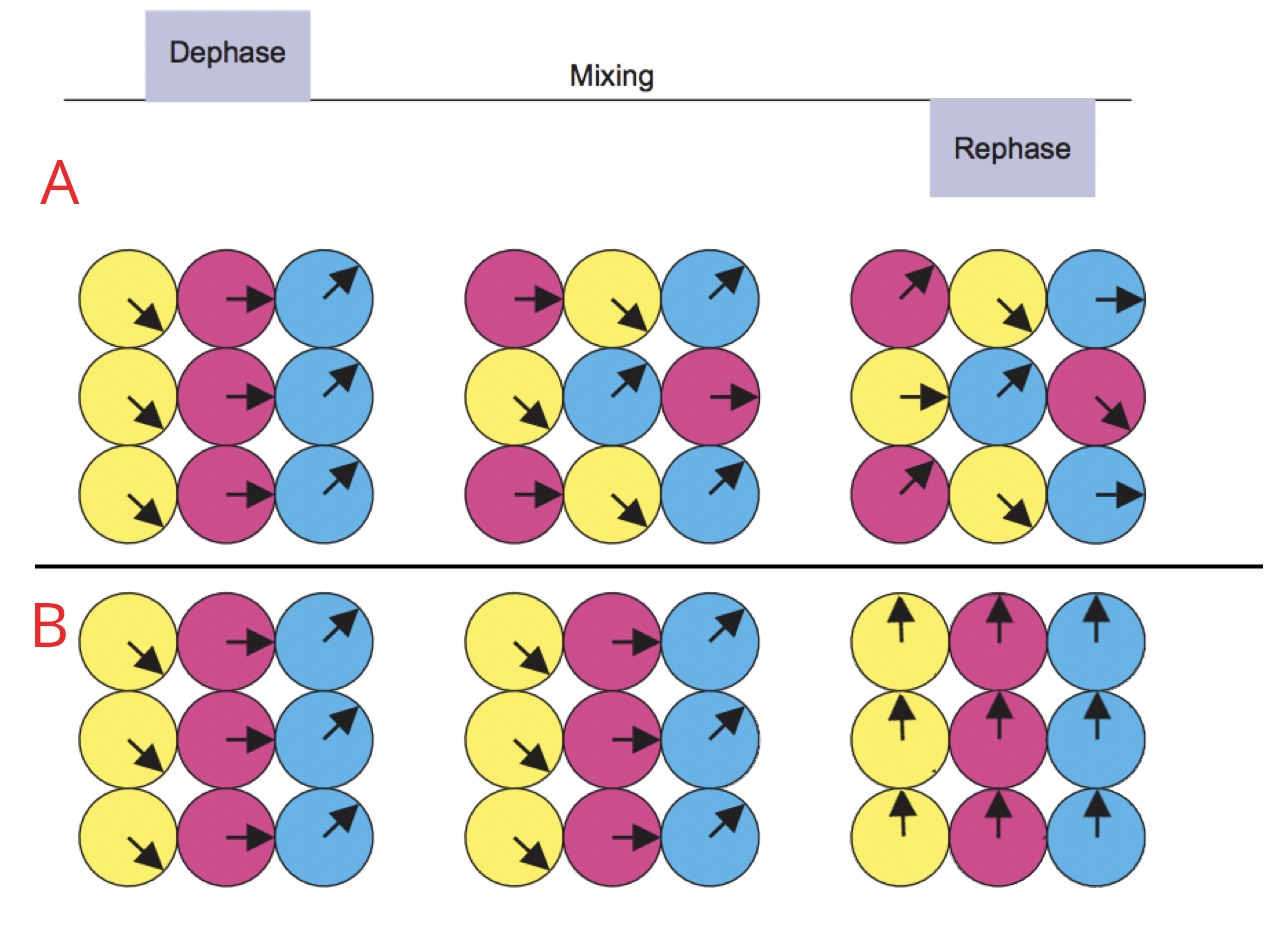
\includegraphics[width=0.5\textwidth]{figures/phase.png}
    \caption{Spin phase of the magnetic moment of nuclei before and after the phase is flipped by a radio sequence pulse. Phase is represented by the arrows and all phases are aligned before the radio pulse, nuclei are coloured based on their initial position. (A) shows the effect diffusion has on the overall phase of the sample compared to (B) which would be the case for completely stationary nuclei. Image adapted from \cite{mori2007introduction}}
    \label{fig:phase}
\end{figure}

\begin{figure}
    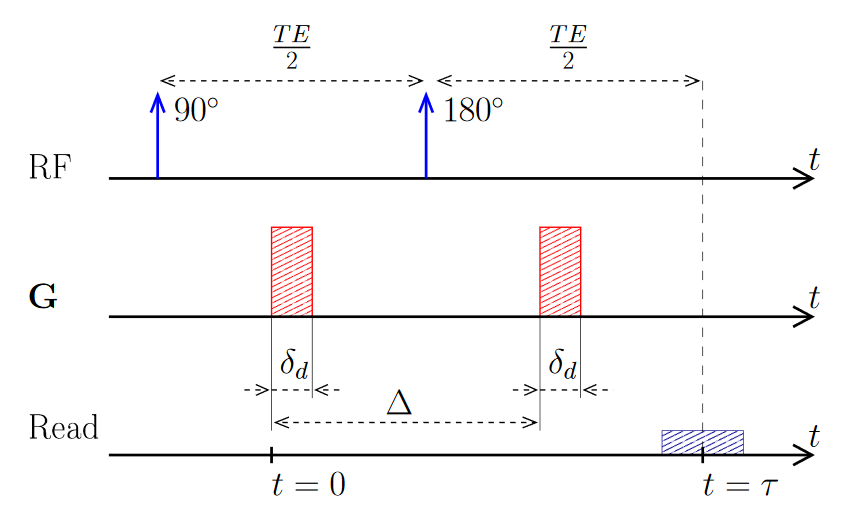
\includegraphics[width=0.5\textwidth]{figures/sequence.png}
    \caption{Visualization of a spin-echo diffusion weighted sequence. Top row gives the timing and phase of the \dmri phasing pulses, center row gives the timing amplitudes and duration of magnetic gradient fields, bottom row approximates the signal from resonating tissue, $\Delta$ can be read as the time between the starts of the gradient pulses, $\delta_d$ can be read as the duration of each gradient pulse, $TE$ is the time between the excitation and collection of an MR signal. Image adapted from \cite{rohmer2006bloch}}.
    \label{fig:sequence}
\end{figure}

\subsection{Biophysical Models of Spinal Cord Microstructure}
Determining the structure of the spinal cord from \dmri data requires fitting the data to a prior model of the microstructure. The ones used in our analysis are:

\subsubsection{Diffusion Tensor Imaging}
\dti is a model where gaussian diffusion is made anisotropic by
 the measured signal is assumed to be given by equation \ref{eq:dti}

\begin{equation}
    S(\hat{g_i}) = S_0 e^{-b \hat{g}_i^T D \hat{g}_i}
    \label{eq:dti}
\end{equation}

Where $D$ is the diffusion tensor, $\hat{g_i}$ is the normalized diffusion gradient, $S_0$ is the expected signal from unrestricted gaussian diffusion. Here the diffusion tensor is a symmetric matrix and therefore requires measuring at least 6 gradient directions to solve for each element. \cite{vedantam2014diffusion}

\subsubsection{Diffusion Kurtosis Imaging}
\dki models non-gaussian diffusion through a Taylor expansion of the signal with respect to the b-value:

\begin{equation}
    \ln[S(b)] = \ln[S(0)] - b D + \frac{b^2}{6} D^2
\end{equation}

Where now $D$ is the kurtosis vector and is represented as a fully symmetric rank 4 tensor which gives 15 independent components. \cite{jensen2005diffusional}

\subsubsection{Spherical Mean Technique}
\smt modelling measures the underlying tissue using data at a fixed b-value using a parameter that is invariant of axon orientation and therefore does not have to make simplifying assumptions about the crossing or dispersion of the fibre anatomy. First we define a normalized diffusion signal:

\begin{equation}
    e_b(\vec{g}) = \frac{S_b(\vec{g})}{S_0}
\end{equation}

We then consider $\bar{e_b}$ which is defined as the spherical mean of $e_b$ averaged over every gradient direction.

\begin{equation}
    \bar{e_b} = \frac{1}{4\pi} \int_{S^2} e_b(\vec{g}) d\vec{g}
\end{equation}

Where the integral is over the surface of a unit sphere. $\bar{e_b}$ is then related to the diffusion coefficient parallel and perpendicular to the axons through:

\begin{equation}
    \bar{e_b} = \exp(-b \lambda_\perp) \cdot
    \frac{\sqrt{\pi}\erf \left(\sqrt{b (\lambda_\parallel - \lambda_\perp)}\right)}
    {2 \sqrt{b (\lambda_\parallel - \lambda_\perp)}}
\end{equation}

Where $0 \leq \lambda_\perp \leq \lambda_\parallel \leq \lambda_\text{free}$, where $\lambda_\perp$ and $\lambda_\parallel$ are the diffusion coefficients perpendicular and parallel to the axons and $\lambda_\text{free}$ is the gaussian diffusion coefficient in the absence of any axons. \cite{kaden2016quantitative}

\subsubsection{Neurite Orientation Dispersion and Density Imaging}
Neurite Orientation Dispersion and Density Imaging (NODDI) is a model that separates the tissue into three compartments: the intracellular region, the extracellular region, and the \csf. The measured signal is modelled as:

\begin{equation}
    S = (1 - \nu_{iso})(\nu_ic S_{ic} + (1- \nu_{ic}) S_{ec}) + \nu_{iso} S_{iso}
\end{equation}

Where $S_{ic}$ and $S_{ec}$ are the diffusion signals due to the intra and extra cellular regions, $S_{iso}$ is the isotropic diffusion in the \csf compartment, and $\nu_{ic}$, $\nu_{ec}$, and $\nu_{iso}$ are their respective volume fractions. The intracellular compartment is modelled as a set of cylinders with zero radius such that diffusion can only occur along its length and is given by:

\begin{equation}
    S_{ic} = \int_{S^2} f(\vec{n}) e^{-b d_\parallel (\vec{g} \cdot \vec{n})^2} d\vec{n}
\end{equation}

Where $f(\vec{n})$ is the orientation density for axons being aligned with the direction of $\vec{n}$ and $d_\parallel$ is the diffusivity of water along the length of the axon. The extracellular component of the signal is modelled as anisotropic gaussian diffusion like that discussed in the \dti section, and $S_{iso}$ is modelled as isotropic diffusion discussed in the \dmri section. \cite{zhang2012noddi}

\subsubsection{Diffusion Basis Spectrum Imaging}
\dbsi is a model where we consider the \dmri signal to be a linear combination of anisotropic compartments and a spectrum of isotropic diffusion tensors where the signal is given by:

\begin{IEEEeqnarray*}{rCl}
    S(\hat{g}_i) &=& \sum_{n=1}^{N_{\text{Aniso}}} f_n e^{-b_i} \lambda_{\perp, n} e^{-b_i (\lambda_{\parallel, n} - \lambda_{\perp, n}) \cos^2(\psi_{i, n})}\\
    && + \int_a^b f(D) e^{-b_i D} dD
\end{IEEEeqnarray*}

Where we need to fit $N_\text{Aniso}$ the number of anisotropic tensors, $\lambda_{\perp, n}$ and $\lambda_{\parallel, n}$ the diffusivities of the nth anisotropic tensor, $a$ and $b$ the diffusivity limits for the diffusion spectrum, $D$, and $f_n$ is the signal intensity fraction for the nth tensor.














\if{false}
Charged particles such as protons that posses a non-zero spin have an intrinsic angular momentum and this gives it a magnetic moment. The presence of a magnetic field lifts the energy degeneracy of the orientation of the magnetic substates of having the spin aligned or anti aligned with the direction of the magnetic field, this is known as the Zeeman effect. Such particles in a magnetic field can absorb or release electro magnetic radiation in order to transition between the two states, such photons have an energy given by the energy separation between the two states.

% Nuclear magnetic resonance.
Consider a large collection of protons in equilibrium with at temperature T, the ratio of spin up to spin down is given by the boltzmann factor and is small even when multiplied by avagadros number, if we choose a magnetic field on the order of a few tesla the frequency involved to get an appreciable energy is on the order of about 100MHz which is radio frequency we need magnetic fields on the order of a few tesla to get to an appreciable energy absorbed.

We can count the number of flipped protons through energy loss in a pickup coil. Scanning a range of radio frequencies and then detecting the resonance where we get the strongest is how one can determine the magnetic moment of the sample.

It turns out that the lamor frequency of atoms is dependent on the chemical environment as protons will feel the applied external field and the internal fields from chemical binding. This change in the lamor frequency gives a shift in the resonant frequencies which can be cataloged into the functional groups. When these are known NMR can be used to identify the functional groups in an unknown sample.

This idea can be inverted if one knows the chemical makeup of the sample a non uniform B field can be applied to the sample such that protons only experience resonance with the provided radio waves at known locations this technique is known as MRI and allows for the mapping of the proton density in various tissues.

\subsubsection{Diffusion MRI}

Unfortunately the MRI technique described above cannot image tissue at the resolutions necessary to directly map out the microscopic structure of cells and intracellular space. We can still probe the structure tissues at these small scales by sensitizing our MRI scheme to be sensitive to the motion of water molecules throughout the tissue.

This relies on the fact that when protons excited by a radio pulse take a finite amount of time to relax, now the actual vector magnetization of the entire sample is given by the Bloch equations which has a precession term for the around the orientation of the magnetic field but also an exponential decay to zero with a time constant known as T2. the component of magnetization also decays exponentially to the rest magnetization with a time constant known as T1. T2 is known as the spin spin relaxation, and T1 is known as the spin lattice relaxation.

The class of MRI techniques that are sensitive to diffusion are known as DMRI and the setup is as follows, a large coil generates a large constant B field across the entire sample, and the smaller coils are used to generate a gradient such that the protons in the water will only resonate with the chosen radio frequency at a single plane running through the material.

In ordinary MRI one  measures the frequency and the phase of the RF photons released by the atoms and this generates a reciprocal space matrix of which taking the fourier transform generates the real space image of the sample. Now when the protons absorb the radio photons they become initially aligned with the magnetic field which is constant over the plane in which they are excited. this adds a term to our Bloch equation making it the Bloch Torrey equation where the additional term is the divergence of gradient of the magnetization after it has been multiplied by a diffusion tensor, this term represents the change in magnetization due to the random motion of protons through the tissue as atoms that were not excited. Solving the BT equation depends on a couple factors such as the echo time, the gradient field amplitude, the gyrometric factor.

The pulse that excites the protons gives them all the same phase and if you wait an appropriate amount of time the protons in that plane will begin to dephase as they diffuse in and out of that plane. A second radio pulse can then be delivered that would negate the phase of the protons in that plane had they remained stationary a comparison to the signal that would be expected from free water probes the form of the diffusion tensor, or even better we can just allow no time for diffusion in this case we isolate the diffusion tensor, since it is a symmetric matrix we need at least 6 measurements to fully solve for it. This is single shot echo planar imaging.

To discuss models of the diffusion we first define b-value as the sensitivity to diffusion. we find this from the scans potential to provide a large rande of phases to MR signals and is found by integrating the gradient strength over the echo times.
\fi


\if{false}
\subsection{MRI and DMRI}
See my old PHYS 473 Notes

\subsection{Diffusion Tensor Imaging}
See Poljanka Johnson's proposal as well as my notes on the review paper

\subsection{Biophysical Tissue Models}
See my notes on the Alexander 2010 and the review paper and the ISMRM video.\\


Alexander 2010 is:
\emph{Orientationally invariant indices of axon di-
ameter and density from diffusion MRI}

In particular the story we are trying to help along is the idea that once we know how to model diffusion in heterogeneous tissue we then need to make the model we are trying to fit something that is clinically practical, in particular the idea is that we need to not have a strong orientation dependence of the patient and we need to minimize the required data to be taken.
\fi

% MRI gives us the proton density
% DMRI gives us the directions in which water can diffuse
% A biophysical model predicts the structure from the diffusion
% What kind of diffusion we may expect from a region of damaged tissue


In this section provide details on the theory  needed to clarify the physics/astophysics behind the proposal. If you are building an ESR spectrometer you would need to explain the Zeeman interaction of an electron in a magnetic field. Use diagrams wherever possible. These can be reused or revised
later for subsequent oral presentations and the thesis. Spend the time now to make up some good ones.
Important  points are: (1) they must be  legible. (2) all axis properly labelled with units  etc. (3)any photos sketches should have a scale built in.   (4) Data point and uncertainties  must  be clearly visible.  

\section{Details on Proposed Experiment/Calculation} 


You will use this section to convince the reviewer that the project is feasible.
Here you should describe in detail what measurements, calculations and or simulations will be made. In the case of  an experiment you should provide a schematic of the apparatus  and a circuit diagram for any electronics that you will need etc.    
When describing equipment give model numbers and any relevant specifications that seem appropriate.
Use figures wherever possible to describe 
the proposed setup, electronics etc. If it is a  computational project then describe the nature of the calculations, give a flow chart,  specify in detail what the simplifications and assumptions that will be made,   etc.  How  will you test  that these assumptions are valid for the purpose you require.


The rules on figures are the same for any scientific document:
\begin{enumerate}
    \item Figures must be numbered.
    \item All the information must be easy to read. {\bf The text in a figure (scales etc) 
    should  be  large enough  so that if the figure were reduced to a single
    column the text would be the size of the regular text in the document.} 
    \item Figures must have a caption which explains 
    what is in the figure. {\bf There should
be enough detail in the caption to understand the figure without
reading the text}. 
\item Every figure must be referred to in the text of the proposal.
\end{enumerate}

The figures do not need to be so polished as for a thesis but they must 
be easily read. You can include them using LATEX or simply append them at the end. 
If you append them at the end put the caption at the bottom of that page 
containing the Figure. 
\begin{figure}[h!]
    \centering
    \caption{Make sure the caption  is detailed enough  to fully understand the figure  without having to read the main  text. Resonant series LCR circuit. The properties of the circuit can be analyzed by (1)  making a sudden  change to an otherwise constant input voltage $V_{in}^0$ or by (2)  driving the circuit with a sinusoidal input  voltage  $V_{in}(t)$ . The voltage across the resistor is  (output voltage from the circuit) is a measure of the current in the circuit. }
    
    \label{fig:LCR}       % Give a unique label to the figure. 
\end{figure}

\section{Resources List}
This project will require access to high resolution DMRI scans of 10 spinal cords that were donated to the International Spinal Cord Injury Biobank by people who died of a spinal cord injury. Computational resources include remote access to the 7T server located in the UBC Life Sciences Center and the following software, 3D Slicer, Spinal Cord Toolbox, Python.

Provide a detailed list of all the resources you will need. e.g. any instruments, equipment materials  and where it will come from. If it is going be bought then indicate the delivery time. Indicate what computing needs for the project and where they will come from.  \cite{albayar2019biomarkers}

\section{Planned Schedule}
Late February
\begin{itemize}
    \item Submit written proposal
    \item Finalize image registration
    \item Prepare proposal talk
\end{itemize}

Early March
\begin{itemize}
    \item Give proposal talk
    \item Analyze parameter maps
    \item Create graphs of \dmri metrics in white and grey matter \roi along the spinal cord.
\end{itemize}

\phantom{more line}\\
\phantom{more line}\\

Late March
\begin{itemize}
    \item Determine relevant correlations between biophysical model parameters and \sci
    \item Prepare progress report and oral defense
\end{itemize}

April
\begin{itemize}
    \item Give oral defence
    \item Finalize and submit the written thesis
\end{itemize}


\if{false}
December
\begin{itemize}
    \item Prepare written and oral proposal.
    \item Familiarize myself with MR theory and analysis techniques of DMR data.
\end{itemize}

January
\begin{itemize}
    \item Familiarize myself with the analysis software such as 3D Slicer and Spinal Cord Toolbox.
    \item Perform registration of MRI data to an atlas and obtain map of diffusion metrics along the length of the spinal cords.
\end{itemize}

February
\begin{itemize}
    \item Identify correlations between diffusion metrics and draw conclusions on SCI histologies.
\end{itemize}

March
\begin{itemize}
    \item Prepare progress report, written thesis, and oral defense.
\end{itemize}

April
\begin{itemize}
    \item Give thesis oral defense presentation and finalize submit written thesis.
\end{itemize}
\fi


%\section{Acknowledgements}


% Finally, make the bibliography
\bibliography{references.bib}
    

\end{document}
%
% ****** End of file  ******